\documentclass[CMPE]{../KGCOEReport}
\usepackage{float}
\usepackage{adjustbox}
\usepackage{pdfpages}
\graphicspath{ {./images/} }

\newcommand{\name}{Mohammed Fareed}
\newcommand{\exerciseNumber}{3}
\newcommand{\exerciseDescription}{Instruction Fetch and Decode Stages}
\newcommand{\dateDone}{March 7, 2024}
\newcommand{\dateSubmitted}{March 10, 2024}

\newcommand{\classCode}{CMPE 260}
\newcommand{\LabSectionNum}{4}
\newcommand{\LabInstructor}{Prof.\ Richard Cliver}
\newcommand{\TAs}{Aubrey Tarmu \\ Henry Bang \\ William Tom}
\newcommand{\LectureSectionNum}{2}
\newcommand{\LectureInstructor}{Prof.\ Marcin Lukowiak}


\begin{document}
\maketitle

\section*{Abstract}

The objective of this exercise was to design and create the Instruction Fetch and Decode stages for a pipelined MIPS architecture. This involved developing several modules to facilitate the fetching of program instructions from memory into the processor and parsing these instructions into commands for execution. The design was tested through various behavioral simulations, post-synthesis and post-implementation timing simulations, and ModelSim waveform simulations, demonstrating successful functionality and compliance with hardware specifications.

\section*{Design Methodology}

\subsection*{Instruction Memory}
The Instruction Memory module was designed as a byte-addressable memory unit capable of storing 1024 bytes. This design choice allows the storage of instructions in a compact format while enabling the assembly of 32-bit instructions from consecutive byte locations. To accommodate the byte-addressable nature while outputting 32-bit words, a concatenation logic was implemented. This logic combines four consecutive bytes starting from the addressed location to form a single 32-bit word. A critical aspect of the design was ensuring that the address bounds were properly checked to prevent out-of-range accesses, which would result in outputting zeros.

\subsection*{Instruction Fetch}
The Instruction Fetch module integrates the Instruction Memory, fetching instructions based on the current value of the program counter (PC). The PC increments by 4 every clock cycle, ensuring sequential instruction fetching. An asynchronous reset feature was implemented to reset the PC to its initial state upon receiving the reset signal. Additionally, the module was designed to handle addresses beyond 1023 (out-of-bounds access) by returning zeros. The out-of-range check was implemented by adding a PC port to the module, which is modified by the testbench to verify the module's behavior under various address conditions. The conditions checked include accessing an instruction that is completely out of range and accessing an instruction that is partially out of range.

\subsection*{Control Unit}
The Control Unit was designed to decode the 32-bit instruction opcode into several control signals necessary for the subsequent stages of the MIPS architecture. This module employs a series of processes, each dedicated to generating a specific control signal based on the opcode and function field inputs. These signals include RegWrite, MemtoReg, MemWrite, ALUControl, ALUSrc, and RegDst, which direct the behavior of the execution, memory access, and write-back stages.

ALUSrc and RegDst are generated based on whether the instruction is an R-type or I-type. The ALUControl signal is generated based on the function field of the instruction for R-type instructions and the opcode for I-type instructions, defaulting to addition for both cases, given that addition is required by ADD, ADDI, store, and load instructions. AND, OR, and XOR share the same ALU operations as their corresponding I-type instructions. The RegWrite, MemWrite, and MemtoReg signals are generated based on whether the instruction is a load/store instruction.

\subsection*{Instruction Decode}
The Instruction Decode stage takes the 32-bit instruction from the Fetch stage and parses it into various signals for execution. This involves integrating the Control Unit to generate the necessary control signals and the Register File from Exercise 2 to access operand registers. The design separates the instruction into opcode, function, and immediate value, and register addresses, which are then used to generate the control signals and register addresses. The Register File is accessed using the register addresses, and the data is passed to the Execute stage. The immediate field is sign-extended to 32 bits and passed to the Execute stage for use in I-type instructions. This stage also takes RegWriteEn, RegWriteData, and RegWriteAddr signals from the previous instruction to write back data to the register file.

\subsection*{Connecting Fetch and Decode Stages}
The fetch and decode stages were simulated separately but their design ensured that they could be connected seamlessly. The Fetch stage outputs a 32-bit instruction each clock cycle, which is then passed to the Decode stage. The Decode stage takes the instruction and generates the necessary control signals and register data for the Execute stage. Figure \ref{fig:fetch_decode} shows the connection between the Fetch and Decode stages.

\begin{figure}[H]
    \centering
    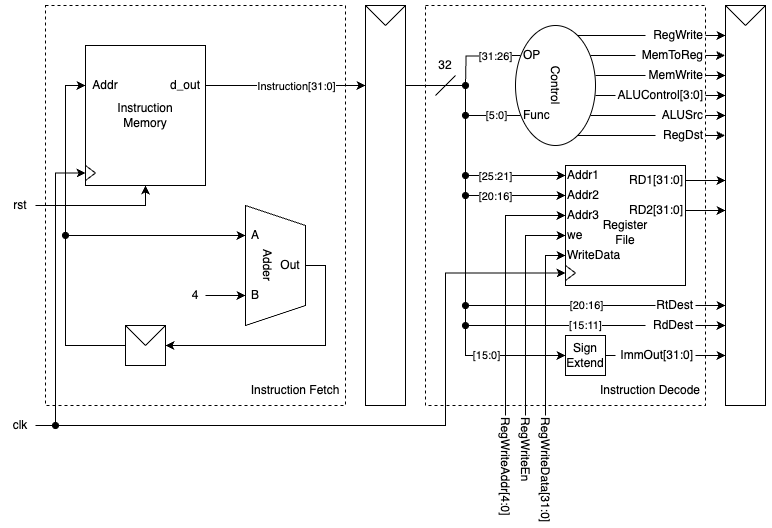
\includegraphics[width=0.791\textwidth]{block_diagram.png}
    \caption{Connection between Fetch and Decode stages}
    \label{fig:fetch_decode}
\end{figure}

The figure shows the connection between the Fetch and Decode stages. The Fetch stage outputs a 32-bit instruction that is disassembled by the Decode stage and fed into the control unit and register file. The control unit generates the necessary control signals for the Execute stage, and the register file accesses the operand registers. All of these signals are then passed to the Execute stage for execution. The figure also shows the data passed into the decode stage from subsequent stages, which is used to write back data to the register file.

\section*{Results and Analysis}

The Instruction Fetch and Decode stages were implemented in VHDL, designed to fit into a pipelined MIPS architecture. For the Instruction Fetch, the primary focus was on accurately fetching program instructions from memory, facilitated by a byte-addressable Instruction Memory module capable of holding 1024 bytes. The Decode stage focused on parsing the fetched instructions into specific commands for subsequent stages. Both stages underwent testing through behavioral simulations, post-implementation timing simulations, and verification against specified test cases to ensure functionality and performance within an FPGA environment.

\subsection*{Instruction Fetch Testing}

The behavioral simulations for the Instruction Fetch stage validated the sequential instruction retrieval and program counter incrementation. Testing also covered the module's response to reset conditions, ensuring the design's compliance with hardware specifications. The test cases for the Instruction Fetch stage are shown in Table \ref{tab:fetch_test_cases}.

\begin{table}[H]
\centering
\begin{tabular}{|c|c|c|}
\hline
\textbf{rst} & \textbf{Address} & \textbf{Fetched Instruction} \\
\hline
1 & 0x00000000 & 0x00000000 \\
0 & 0x00000004 & 0x11111111 \\
0 & 0x00000008 & 0x22222222 \\
0 & 0x0000000C & 0x1f2e3d4c \\
0 & 0x00000010 & 0x12345678 \\
0 & 0x00000014 & 0x00000001 \\
0 & 0x00000018 & 0x00000002 \\
0 & 0x0000001C & 0x00000003 \\
0 & 0x00000020 & 0x5a5a5a5a \\
1 & 0x00000000 & 0x00000000 \\
0 & 0x00000004 & 0x11111111 \\
0 & 0x00000008 & 0x22222222 \\
\hline
\end{tabular}
\caption{Instruction Fetch Simulation Test Cases}
\label{tab:fetch_test_cases}
\end{table}

The test cases fetch consecutive instructions from the Instruction Memory starting at the beginning of memory through applying a reset signal, verifying the module's ability to fetch instructions sequentially and increment the program counter. The reset signal is then applied again to verify the module's response to reset conditions. Figure \ref{fig:behave_fetch} shows the waveform of the behavioral simulation of the Instruction Fetch stage.

\begin{figure}[H]
    \centering
    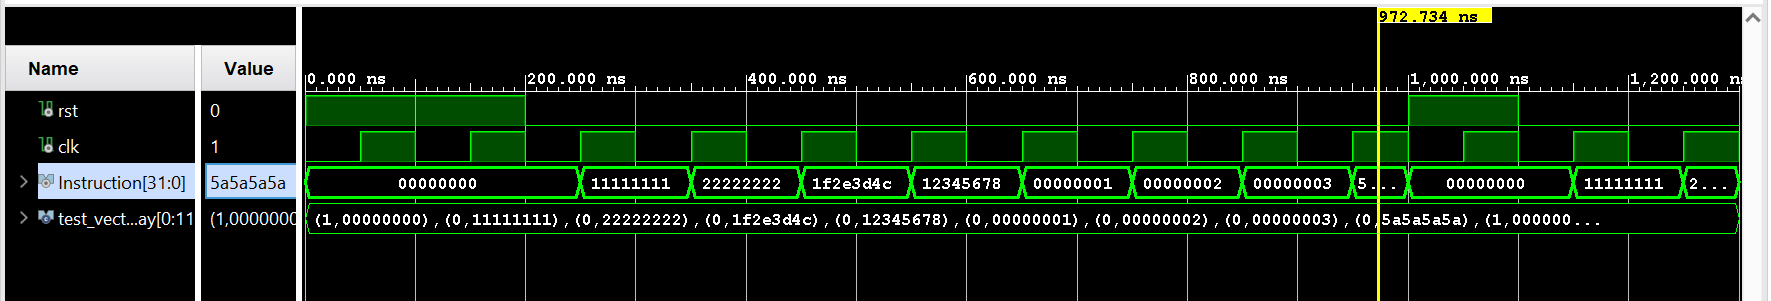
\includegraphics[width=1\textwidth]{behave_fetch.png}
    \caption{Waveform of behavioral simulation ofInstruction Fetch stage}
    \label{fig:behave_fetch}
\end{figure}

The figure shows that the Instruction Fetch stage successfully fetches instructions from the Instruction Memory and increments the program counter sequentially according to the instructions specified in Table \ref{tab:fetch_test_cases}. The module also responds correctly to the reset signal, resetting the program counter to its initial state asynchronously, resulting in 0x00000000 being fetched from the Instruction Memory, followed by the next instructions in the sequence shown in Table \ref{tab:fetch_test_cases}.
\\

Post-implementation timing simulation was then performed to evaluate the module's performance under FPGA conditions. The simulation results are shown in Figure \ref{fig:implement_fetch}.

\begin{figure}[H]
    \centering
    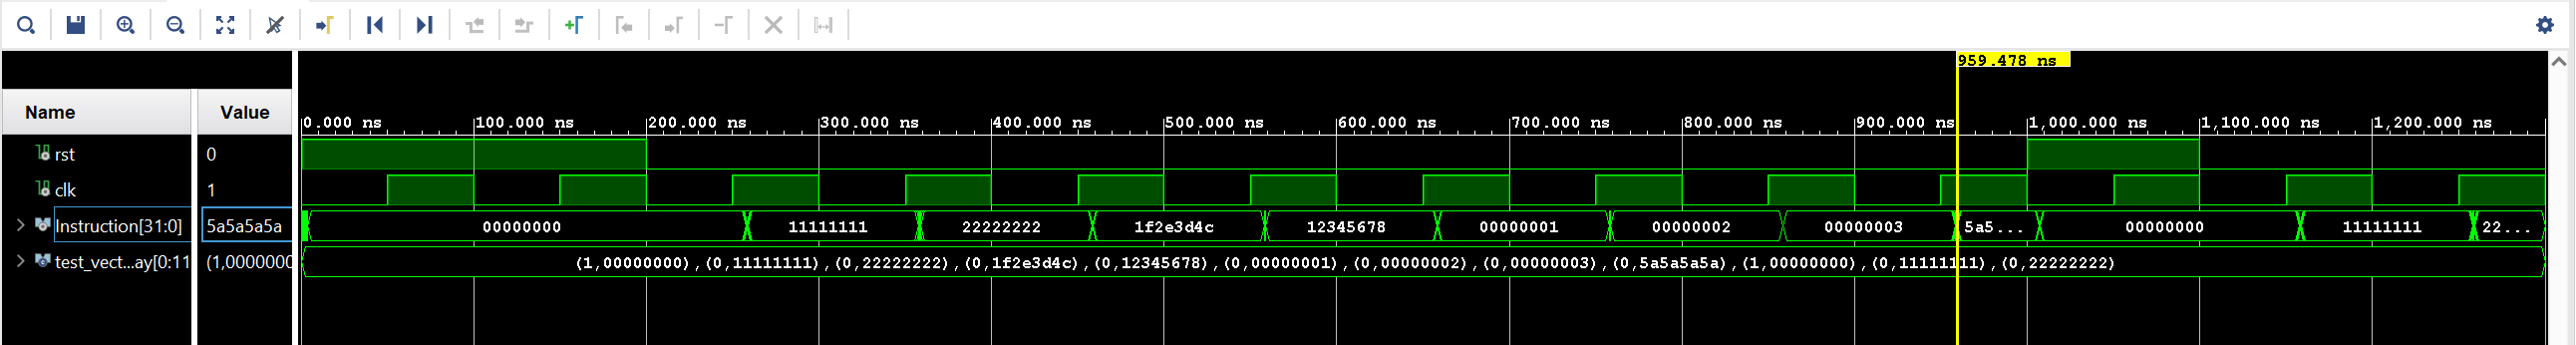
\includegraphics[width=1\textwidth]{implement_fetch.png}
    \caption{Waveform of post-implementation timing simulation of Instruction Fetch stage}
    \label{fig:implement_fetch}
\end{figure}

The timing simulation results shown above demonstrate the module's compliance with timing and functional requirements. The simulation shows response times well within the specified clock cycle. It also shows an average delay of 9.5ns for the module to fetch an instruction from the Instruction Memory and increment the program counter.
\\

The final step in testing the Instruction Fetch stage was to verify its functionality through ModelSim waveform simulations. The results of the ModelSim simulation are shown in Figure \ref{fig:modelsim}.

\begin{figure}[H]
    \centering
    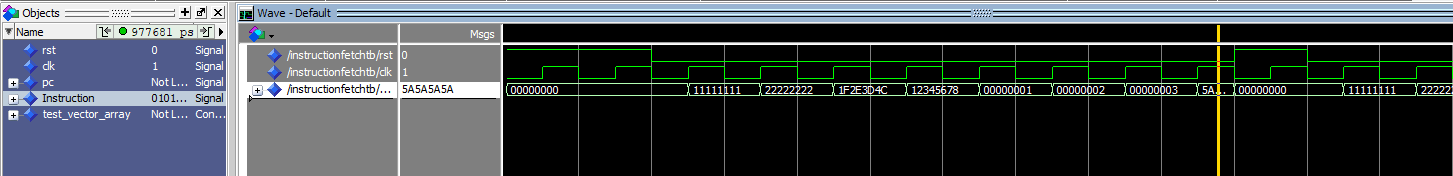
\includegraphics[width=1\textwidth]{modelsim.png}
    \caption{Waveform of ModelSim simulation of Instruction Fetch stage}
    \label{fig:modelsim}
\end{figure}

The ModelSim simulation results demonstrate the successful functionality of the Instruction Fetch stage. The waveform shows identical behavior to the behavioral and post-implementation timing simulations, confirming the module's ability to fetch instructions from the Instruction Memory and increment the program counter sequentially.
\\

Out-of-bounds access was also tested by modifying the PC port of the Instruction Fetch module to access instructions beyond the 1020 to 1023 instruction then using assert statements to verify that the module returns zeros for out-of-bounds access. The indices tested were 1022, which is partially out of range, and 1024, which is completely out of range. The module correctly returned zeros for the out-of-bounds access, without resulting in any errors or warnings due to the assert statements.

\subsection*{Instruction Decode Testing}

Following the successful simulation of the Instruction Fetch, the Instruction Decode stage was tested. This stage's capability to decode fetched instructions into a set of actionable signals for the execution stage was verified. Table \ref{tab:decode_test_cases} shows the test cases for the Instruction Decode stage.

\begin{table}[H]
\centering
\begin{tabular}{|c|c|c|c|c|}
\hline
\textbf{Instruction} & \textbf{RegWriteEn} & \textbf{RegWriteAddr} & \textbf{RegWriteData} & \textbf{Expected Output} \\
\hline
0x00000000 & '1' & 0x00 & 0x00000000 & NOOP \\
0x00211020 & '1' & 0x01 & 0x12121212 & ADD R1, R1, R2 \\
0x2021000D & '1' & 0x02 & 0x00000001 & ADDI R1, R1, 13 \\
0x8C410000 & '1' & 0x01 & 0x00000000 & LW R1, 0(R2) \\
0x00411000 & '1' & 0x02 & 0x00000000 & SLL R1, R2, 2 \\
\hline
\end{tabular}
\caption{Instruction Decode Simulation Test Cases}
\label{tab:decode_test_cases}
\end{table}

The test cases specified above cover a range of instructions, including R-type, I-type, and load/store instructions. The instructions are decoded into control signals and register data, which are then passed to the Execute stage. They also test writing back to the register file by writing data to registers then reading the data back in subsequent instructions. Figure \ref{fig:behave_decode} shows the waveform of the behavioral simulation of the Instruction Decode stage.

\begin{figure}[H]
    \centering
    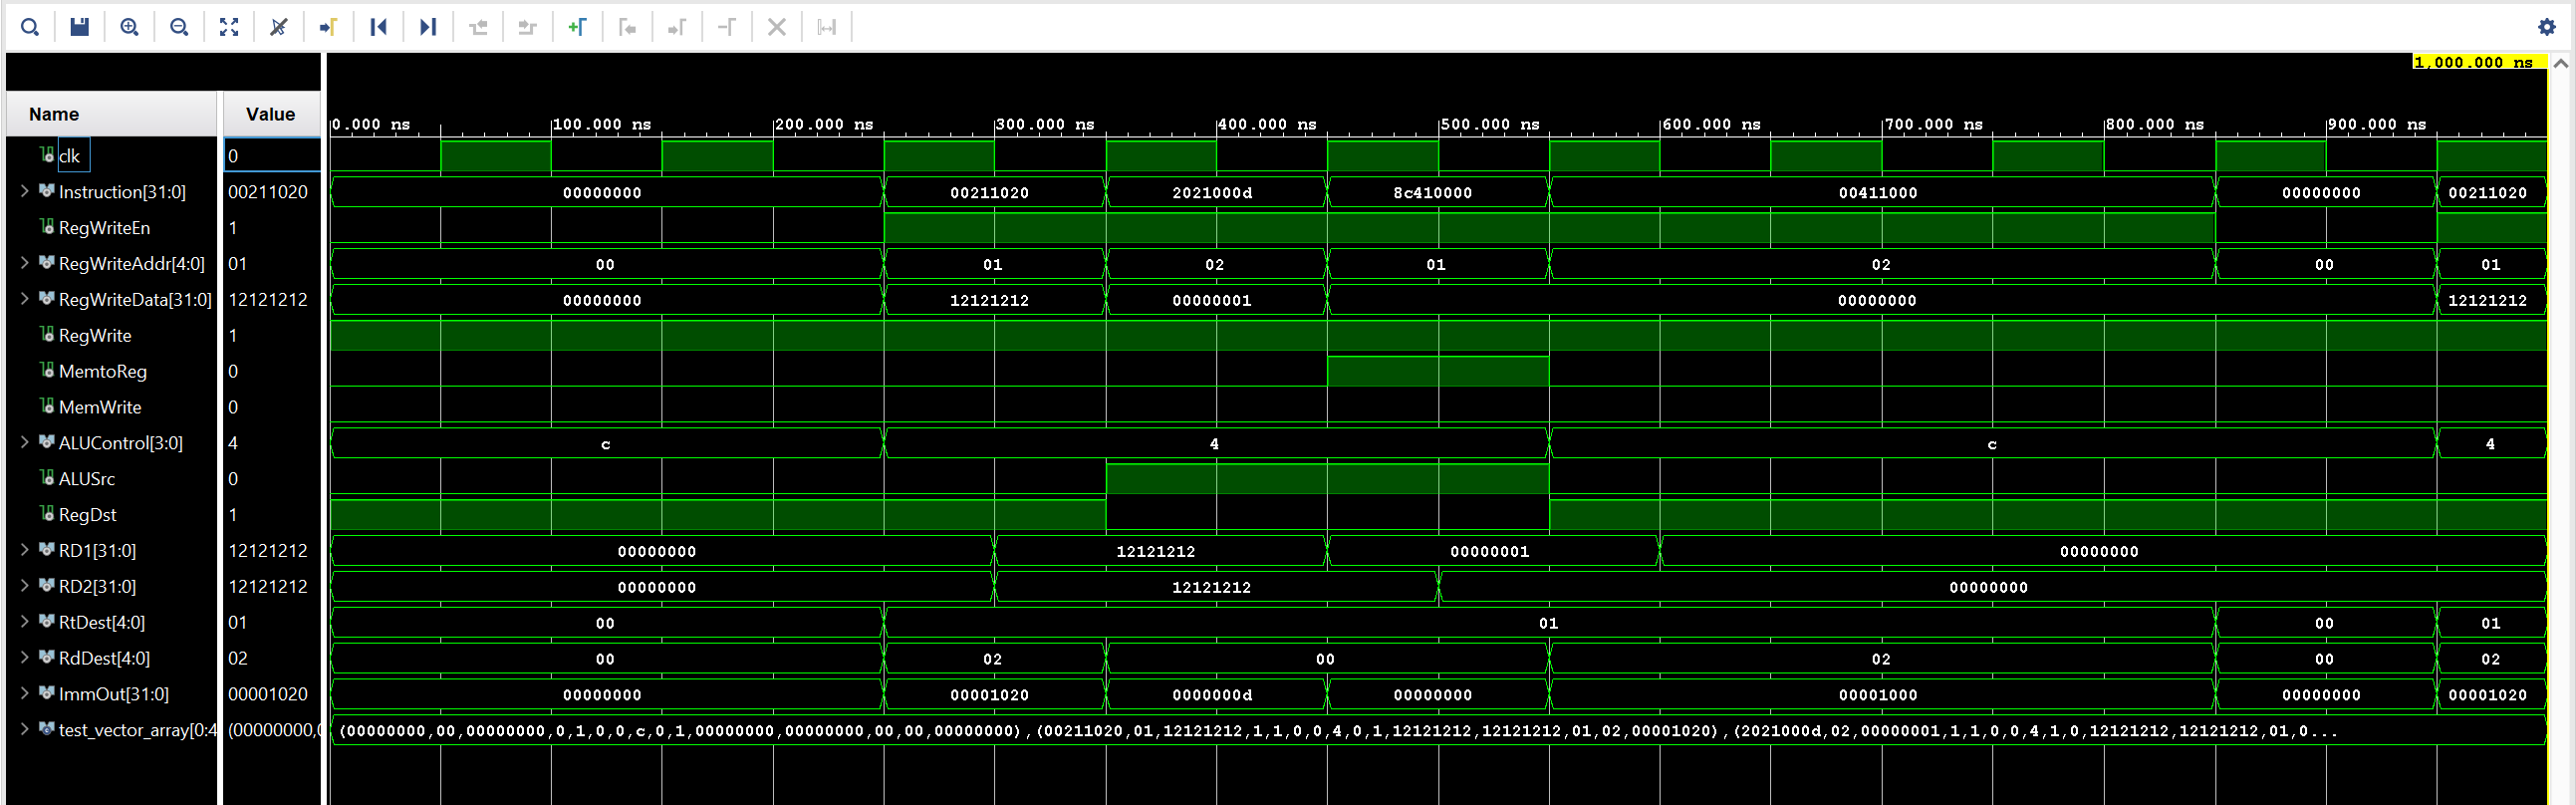
\includegraphics[width=1\textwidth]{behave_decode.png}
    \caption{Waveform of behavioral simulation of Instruction Decode stage}
    \label{fig:behave_decode}
\end{figure}

The figure shows that the Instruction Decode stage successfully decodes the instructions specified in Table \ref{tab:decode_test_cases} into control signals and register data. The waveform shows at 250ns that the \verb|ADD R1, R1, R2| results in the value 0x12121212 being written to register 1, then decoded into RD1 and RD2, demonstrating correct behavior of the register file. The signals RegWrite and RegDst are correctly set for the instruction. The ALUControl signal is also correctly set to 0b0100 for the ADD instruction with ALUSrc correctly set to 0. The Rt and Rd registers were correctly decoded to 1 and 2 respectively. Lastly, the immediate value was correctly sign-extended to 32 bits as 0x00001020, which is correctly (first 16 bits of the instruction) although not used. The NOOP instruction is also decoded correctly, resulting in no control signals being generated.
\\

Post-implementation timing simulation was then performed to evaluate the module's performance under FPGA conditions. The simulation results are shown in Figure \ref{fig:implement_decode}.

\begin{figure}[H]
    \centering
    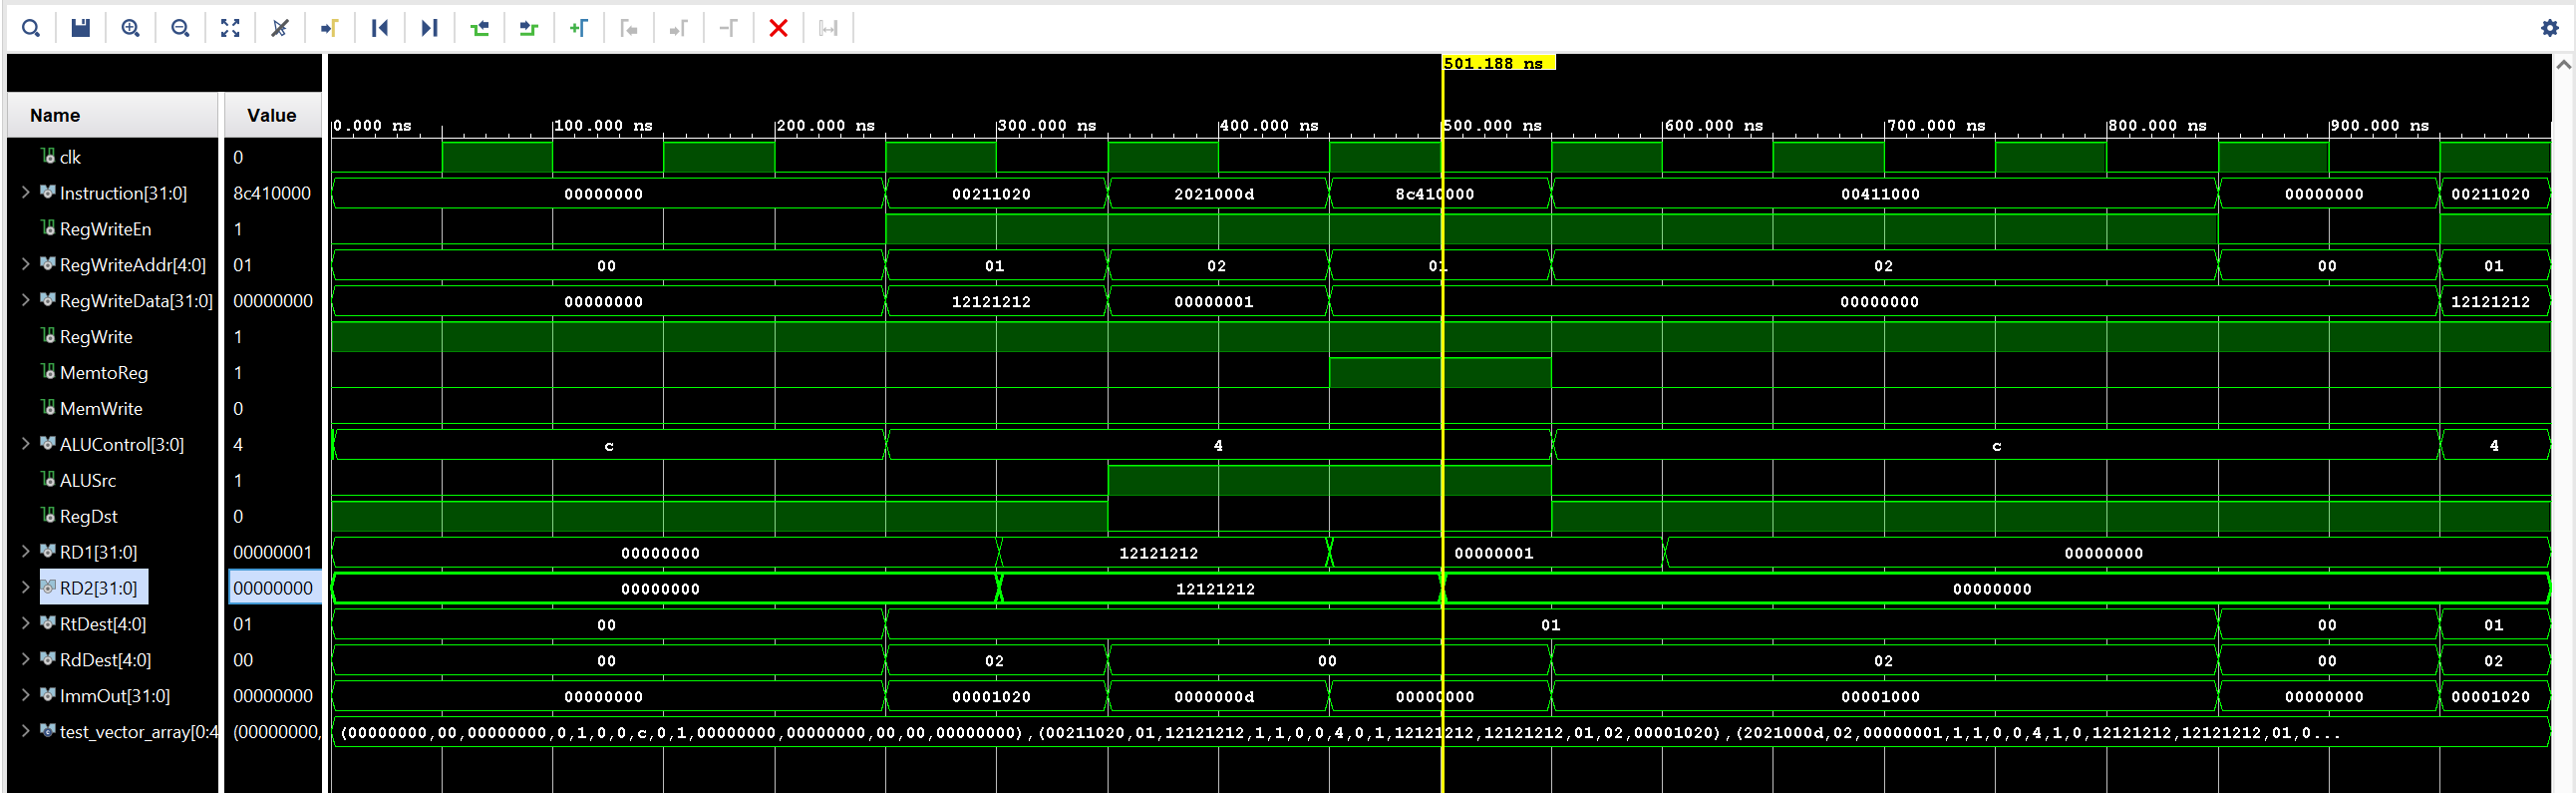
\includegraphics[width=1\textwidth]{implement_decode.png}
    \caption{Waveform of post-implementation timing simulation of Instruction Decode stage}
    \label{fig:implement_decode}
\end{figure}

The timing simulation results shown above demonstrate the module's compliance with timing and functional requirements. The simulation shows response times well within the specified clock cycle. It also shows an average delay of 1.5ns for the module to decode an instruction into control signals and register data.

\section*{Conclusion}

The design and implementation of the Instruction Fetch and Decode stages for a pipelined MIPS architecture were successfully completed. The Instruction Fetch stage was designed to fetch program instructions from memory, incrementing the program counter sequentially and responding to reset conditions. The Instruction Decode stage was designed to parse the fetched instructions into control signals and register data for the Execute stage. Both stages were tested through behavioral simulations, post-implementation timing simulations, and ModelSim waveform simulations, demonstrating successful functionality and compliance with hardware specifications. The results of the simulations confirmed the correct operation of the Instruction Fetch and Decode stages, with delays within the expected range, ensuring the design's performance and timing.

\newpage
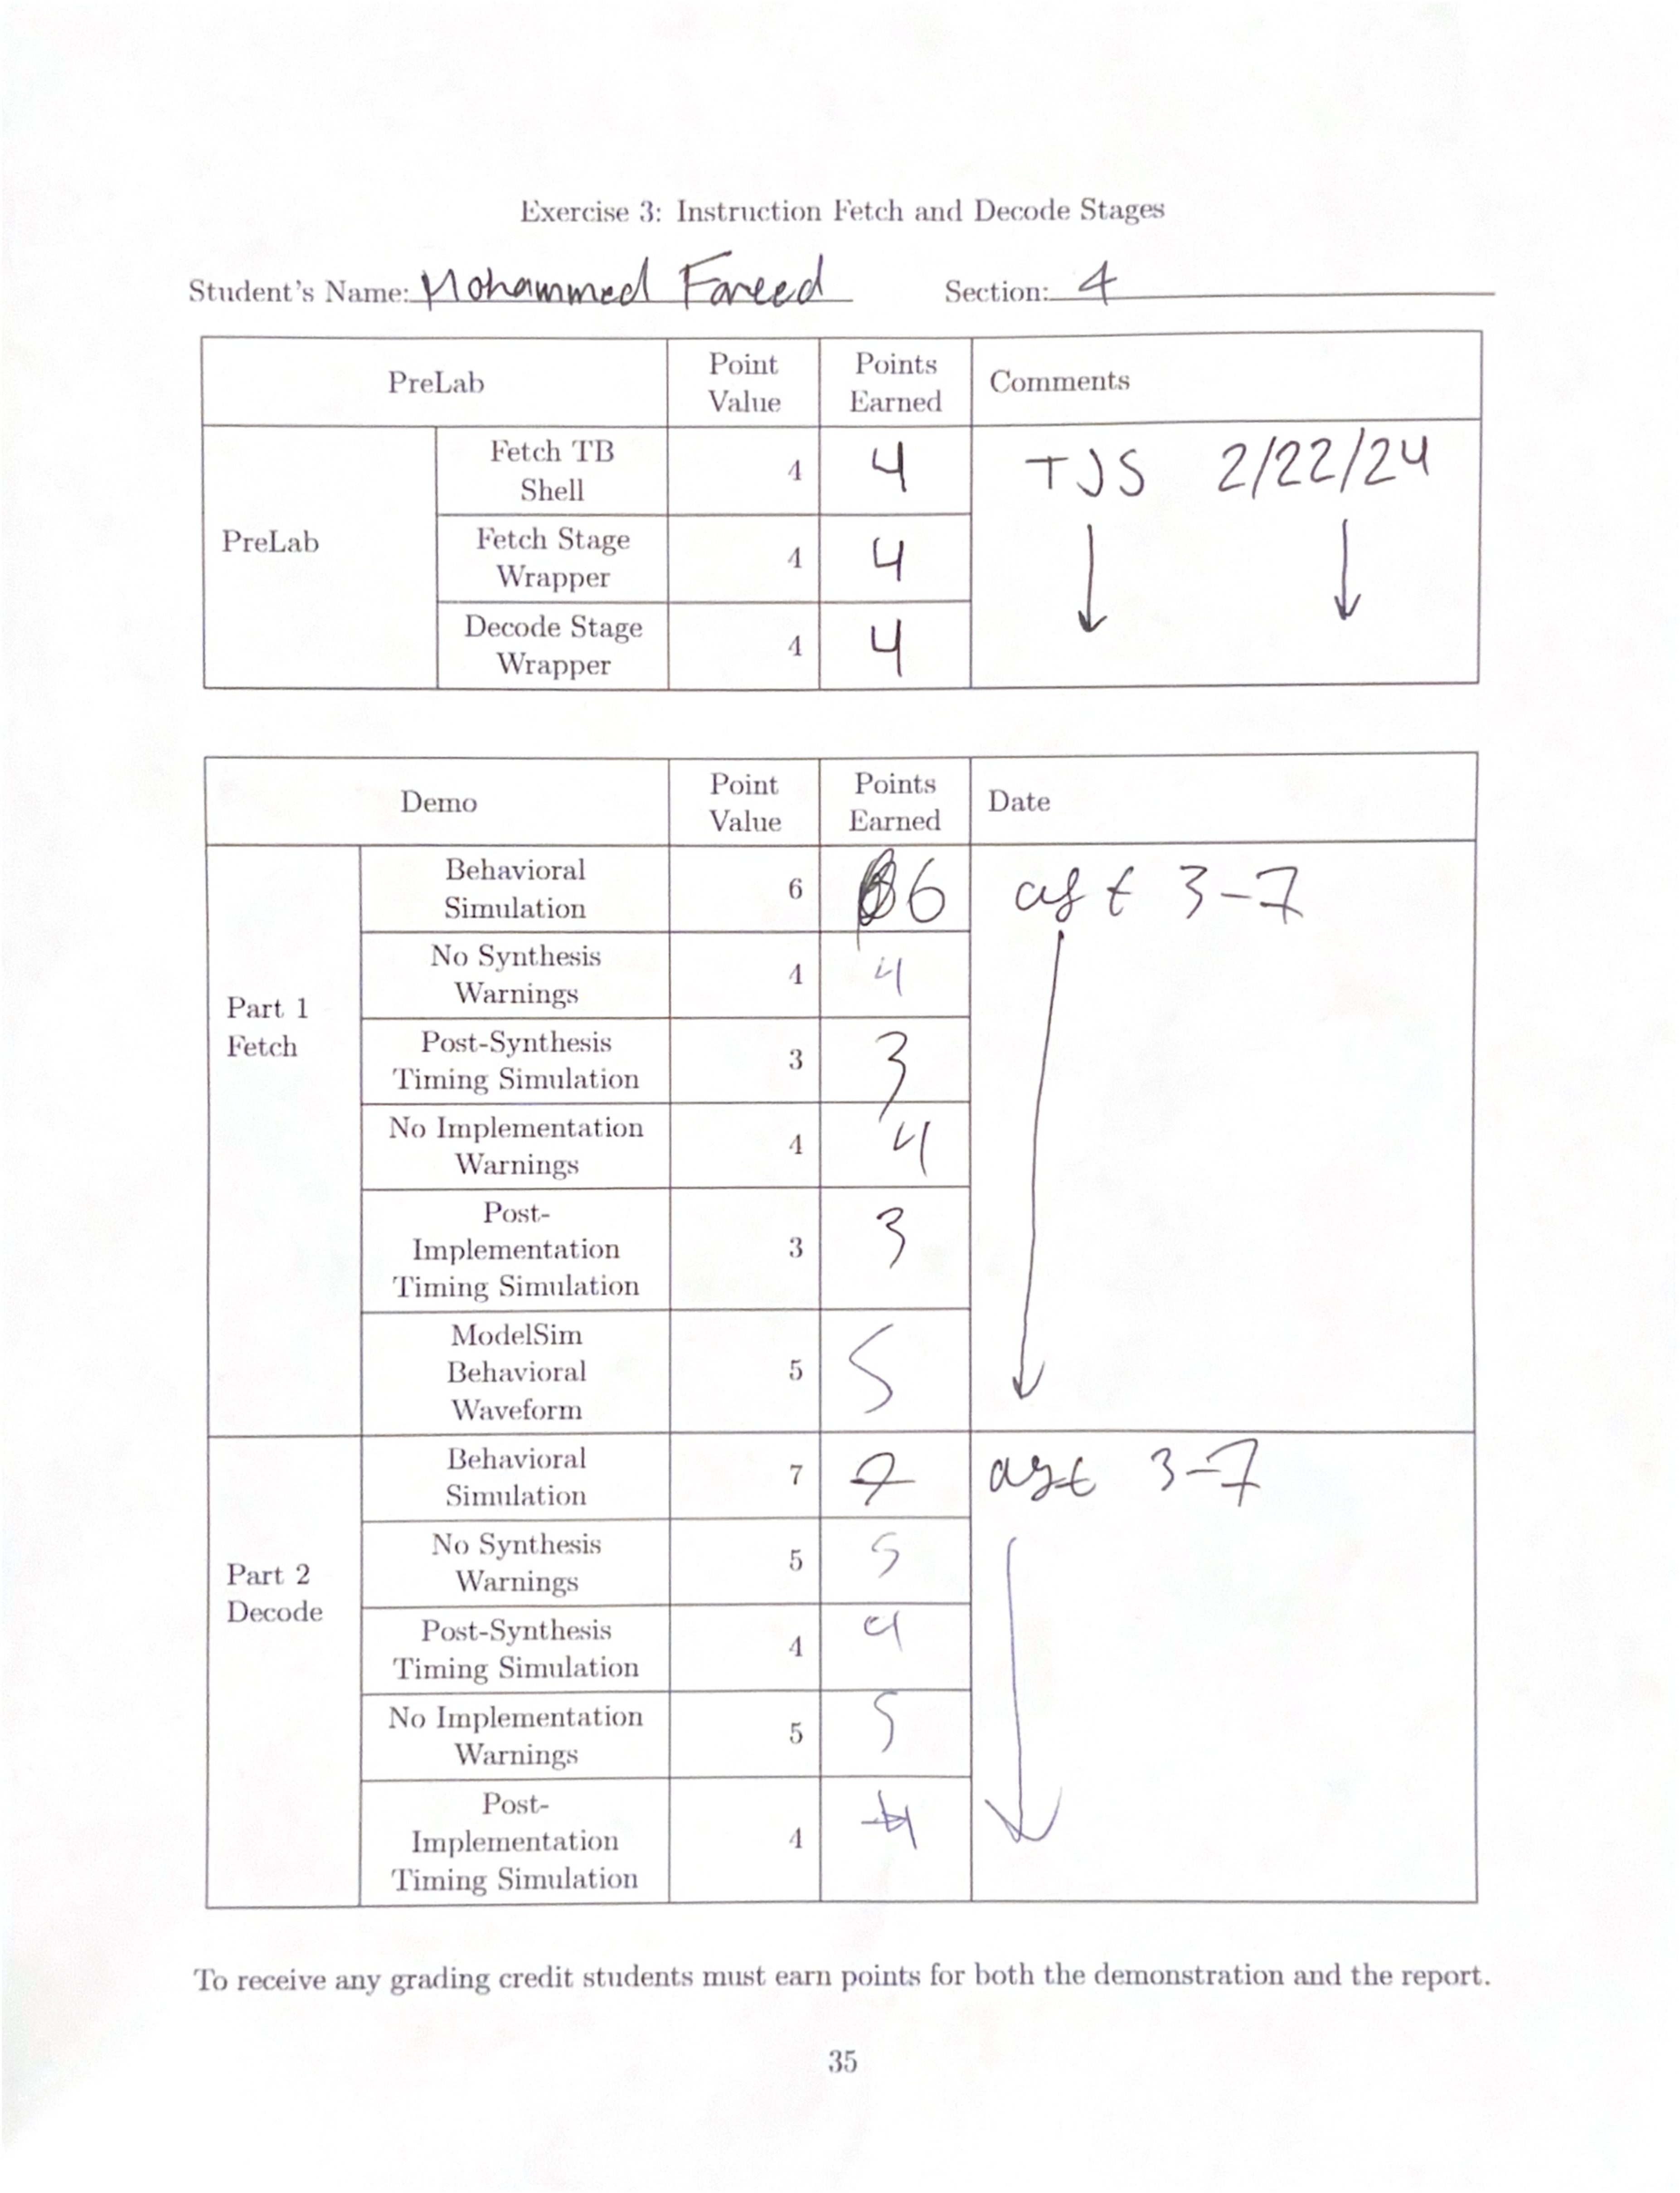
\includepdf[pages=-]{signoff.pdf}

\end{document}
